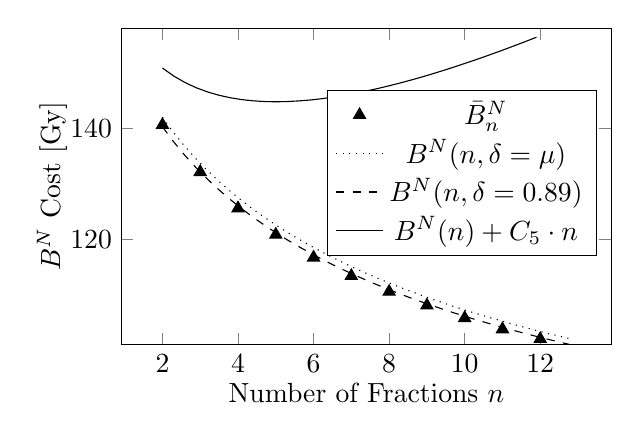
\begin{tikzpicture}
    \begin{axis}
    [
        ymin=101,
        ymax=158,
        xlabel={Number of Fractions $n$}, 
        ylabel={$B^{\text{N}}$ Cost [Gy]},
        ylabel style=
        {
        yshift=-2mm
        },
        xlabel style=
        {
        yshift=+1mm
        },
        legend style={at={(axis cs:13.5,117)}, anchor=south east},
        width=7.8cm,
        height=5.6cm
    ]  
    \addplot[only marks, mark=triangle*, mark size=2.5pt]
        coordinates {
            (2.0, 140.58)
            (3.0, 132.1)
            (4.0, 125.55)
            (5.0, 120.81)
            (6.0, 116.69)
            (7.0, 113.37)
            (8.0, 110.53)
            (9.0, 108.06)
            (10.0, 105.78)
            (11.0, 103.77)
            (12.0, 102.02)
        };
    \addlegendentry{$\bar{B}_n^{\text{N}}$}

    \addplot[no marks, dotted]
        coordinates {
            (2.0, 141.96)
            (2.3, 139.17)
            (2.6, 136.66)
            (2.9, 134.39)
            (3.2, 132.3)
            (3.5, 130.38)
            (3.8, 128.6)
            (4.1, 126.94)
            (4.4, 125.38)
            (4.7, 123.93)
            (5.0, 122.56)
            (5.3, 121.26)
            (5.6, 120.04)
            (5.9, 118.87)
            (6.2, 117.77)
            (6.5, 116.72)
            (6.8, 115.71)
            (7.1, 114.75)
            (7.4, 113.84)
            (7.7, 112.96)
            (8.0, 112.11)
            (8.3, 111.3)
            (8.6, 110.53)
            (8.9, 109.78)
            (9.2, 109.05)
            (9.5, 108.36)
            (9.8, 107.68)
            (10.1, 107.03)
            (10.4, 106.41)
            (10.7, 105.8)
            (11.0, 105.21)
            (11.3, 104.64)
            (11.6, 104.09)
            (11.9, 103.55)
            (12.2, 103.03)
            (12.5, 102.53)
            (12.8, 102.04)
        };
    \addlegendentry{$B^{\text{N}}(n, \delta=\mu)$}
    
    \addplot[no marks, dashed]
        coordinates {
            (2.0, 140.25)
            (2.3, 137.51)
            (2.6, 135.04)
            (2.9, 132.8)
            (3.2, 130.75)
            (3.5, 128.86)
            (3.8, 127.11)
            (4.1, 125.48)
            (4.4, 123.95)
            (4.7, 122.52)
            (5.0, 121.17)
            (5.3, 119.89)
            (5.6, 118.69)
            (5.9, 117.55)
            (6.2, 116.46)
            (6.5, 115.43)
            (6.8, 114.44)
            (7.1, 113.5)
            (7.4, 112.59)
            (7.7, 111.73)
            (8.0, 110.9)
            (8.3, 110.1)
            (8.6, 109.34)
            (8.9, 108.6)
            (9.2, 107.89)
            (9.5, 107.2)
            (9.8, 106.54)
            (10.1, 105.9)
            (10.4, 105.29)
            (10.7, 104.69)
            (11.0, 104.11)
            (11.3, 103.55)
            (11.6, 103.01)
            (11.9, 102.48)
            (12.2, 101.97)
            (12.5, 101.47)
            (12.8, 100.99)
        };
    \addlegendentry{$B^{\text{N}}(n, \delta=0.89)$}
    
    \addplot[no marks, solid]
        coordinates {(2.0, 150.83)
            (2.3, 149.38)
            (2.6, 148.21)
            (2.9, 147.26)
            (3.2, 146.51)
            (3.5, 145.92)
            (3.8, 145.47)
            (4.1, 145.14)
            (4.4, 144.92)
            (4.7, 144.79)
            (5.0, 144.75)
            (5.3, 144.79)
            (5.6, 144.9)
            (5.9, 145.06)
            (6.2, 145.29)
            (6.5, 145.57)
            (6.8, 145.9)
            (7.1, 146.27)
            (7.4, 146.69)
            (7.7, 147.14)
            (8.0, 147.63)
            (8.3, 148.15)
            (8.6, 148.7)
            (8.9, 149.28)
            (9.2, 149.89)
            (9.5, 150.53)
            (9.8, 151.19)
            (10.1, 151.87)
            (10.4, 152.57)
            (10.7, 153.3)
            (11.0, 154.04)
            (11.3, 154.8)
            (11.6, 155.58)
            (11.9, 156.38)
        };
    \addlegendentry{$B^{\text{N}}(n) + C_5 \cdot n$}
    
    \end{axis}
\end{tikzpicture}